%%Talk about the replication of the original experiment in a dynamic scenario

The first independent replication to collect empirical results was done with the algorithms proposed in the original work by \textit{Schwarzrock et al.}\cite{MAS07} using the dynamic context presented in Section \ref{sec:dynamic_scenario}. It aims to find evidence to either support or refute the conjecture made in the referenced study that it would be fully functional in dynamic contexts. 

Table \ref{table:table01} shows the results from all experimental scenarios listed in Section \ref{sec:method}. These results show the total reward obtained with the completed tasks, the total tasks finished , the portion of total time ($[0\%,1\%]$) used to perform the maximum possible tasks, the total quality that relates sensors and tasks performed, and the number of tokens sent during the algorithms running. 

\begin{table}%[ht]
	\small
	\fontsize{6}{6}\selectfont
	\centering
	\caption{Total reward, elapsed time, quantity and quality of the completed tasks and number of exchanged messages(tokens sent) for 100 runs of each algorithm with the following attributes: 9 UAVs and 96 tasks in area of 300x240 pixels with deadline of 300 ticks.}
	\label{table:table01}
	
	\begin{tabular}{rrrrr} \hline
		& AL
		& SAL
		& LAL \\ \hline 
		
		& Mean (St.Dev.)  & Mean (St.Dev.)  & Mean (St.Dev.)  \\ [1ex]
		
		\multicolumn{5}{l}{\textbf{Results of the reference study in the same original static context}} \\
	Total reward           & 16.724   ($\pm$2.1908)  & 37.9608  ($\pm$1.1119) & 44.733  ($\pm$1.5961)   \\
	Elapsed time (norm)    & 0.9894   ($\pm$0.0064)  &  0.9763  ($\pm$0.0092) & 0.9693  ($\pm$0.0124)    \\ 
	Comp. tasks (norm)     & 0.2774   ($\pm$0.0276)  &  0.4674  ($\pm$0.0170) & 0.5226  ($\pm$0.0162)    \\ 
	Quality (norm)         & 0.7865   ($\pm$0.0641)  &  0.9680  ($\pm$0.0202) & 0.9752  ($\pm$0.0159)   \\ 
	Sending token          &  9.8667  ($\pm$1.1958)  &  9.7000  ($\pm$1.2360) & 51.500 ($\pm$1.4797)   \\ [1ex]
		
		\multicolumn{5}{l}{\textbf{Independent replication using the dynamic context (number of UAVs changes)}} \\
	Total reward           & 8.6995  ($\pm$1.9489)  & 23.6496 ($\pm$2.6004) &  28.348  ($\pm$2.8464)  \\
	Elapsed time (norm)    & 0.9767  ($\pm$0.0135)  & 0.9652  ($\pm$0.0220) &  0.9513  ($\pm$0.0281)  \\ 
	Comp. tasks (norm)     & 0.1418  ($\pm$0.0281)  & 0.2852  ($\pm$0.0315) &  0.3278  ($\pm$0.0328)  \\ 
	Quality (norm)         & 0.5753  ($\pm$0.1421)  & 0.5751  ($\pm$0.1358) &  0.5858  ($\pm$0.1424)  \\ 
	Sending token          & 10.0900 ($\pm$1.3416)  & 9.9800  ($\pm$1.1805) &  49.4600 ($\pm$1.9562)  \\ [1ex]

		\hline
	\end{tabular}
\end{table} 






We concentrated our analysis in all results of the experiments that used more agents (9 UAVs) and tasks (96) since they represent the highest value difference among the original study and those obtained in dynamic context. Overall, these results suggest that the original algorithms work in dynamic context. Nevertheless, of those results were significantly different from the values obtained by the original work.

In the following, we present and discuss graphs comparing the results of this first replication in the dynamic context (Section \ref{sec:dynamic_scenario}) with the reproduction of original study in the static context (Section \ref{sec:reproducibility}).

Finished tasks (Figure \ref{fig:fig04}) presented a reduction greater than $40\%$ due to the fact that there are fewer agents performing the mission. Indeed, as the dynamic context makes the number of agents decreases in runtime, not all tasks allocated are completed and helps to enhance this difference. 

Another attribute that suffered a significant degradation (greater than $30\%$) was the quality as seen in Figure \ref{fig:fig03}. It was in consequence of the algorithms characteristics that simply discard the tasks allocated, from the available tasks list, when the agent is taken down. These tasks are not reallocated among the remaining UAVs, thus reducing the quality of sensors related to finished tasks.

The quality attribute is important because it impacts on the agent capability ($k_{ij}$) and this variable correlates the sensors characteristics and the type of task showing how suitable the sensor is to perform a specific task. 

\begin{figure}[h!]
	\begin{center}
		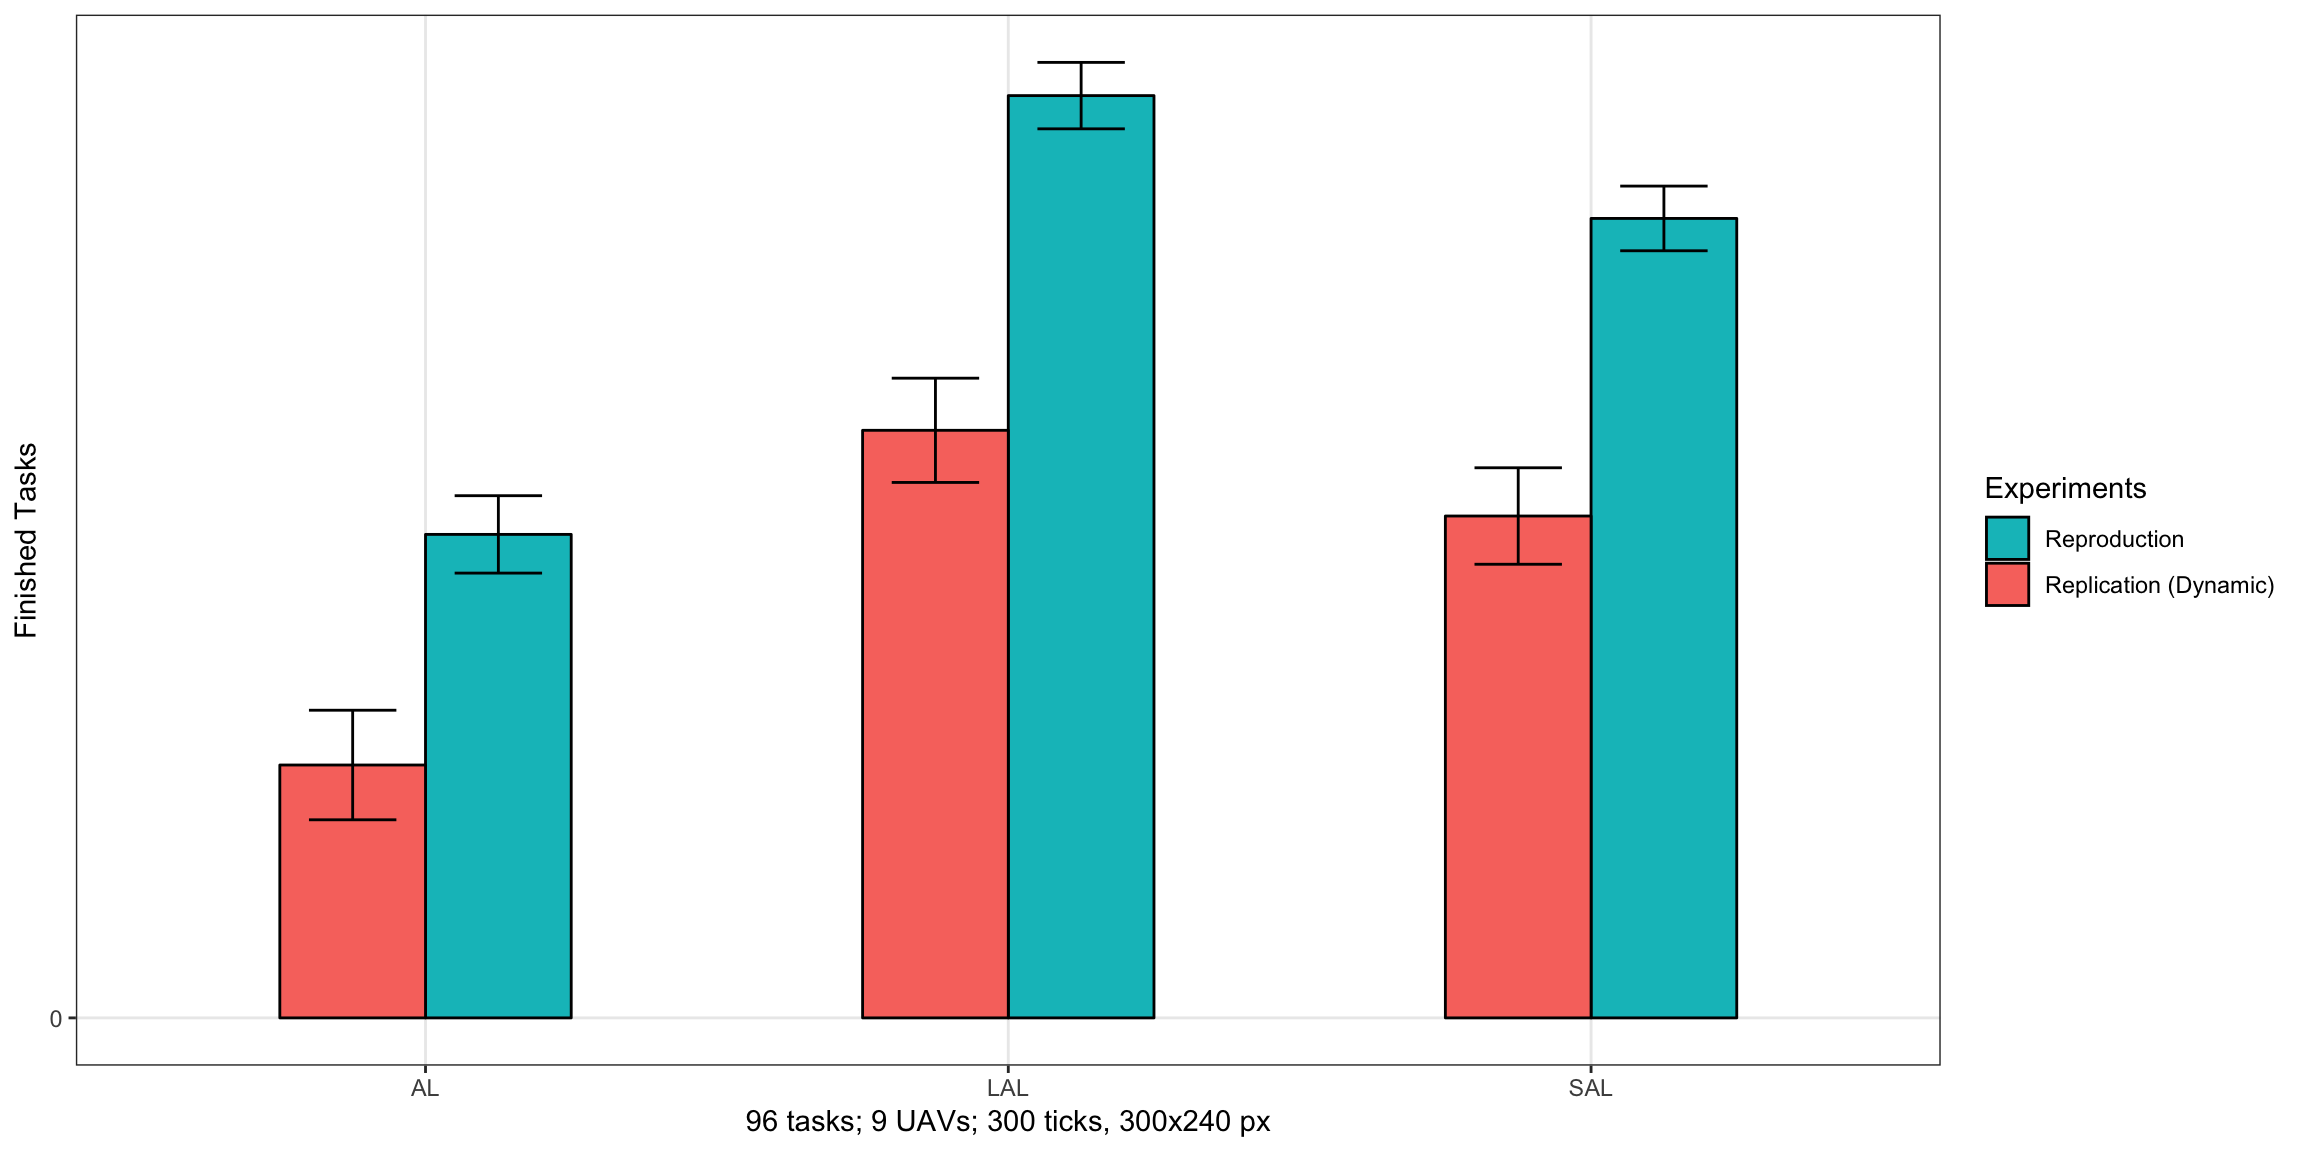
\includegraphics[scale=0.15]{fig/finished_orig.png}
		\caption{Finished Tasks (96 tasks; 9 UAVs; 300 x 240; 300 ticks)}
		\label{fig:fig04}
	\end{center}
\end{figure}

\begin{figure}[h!]
	\begin{center}
		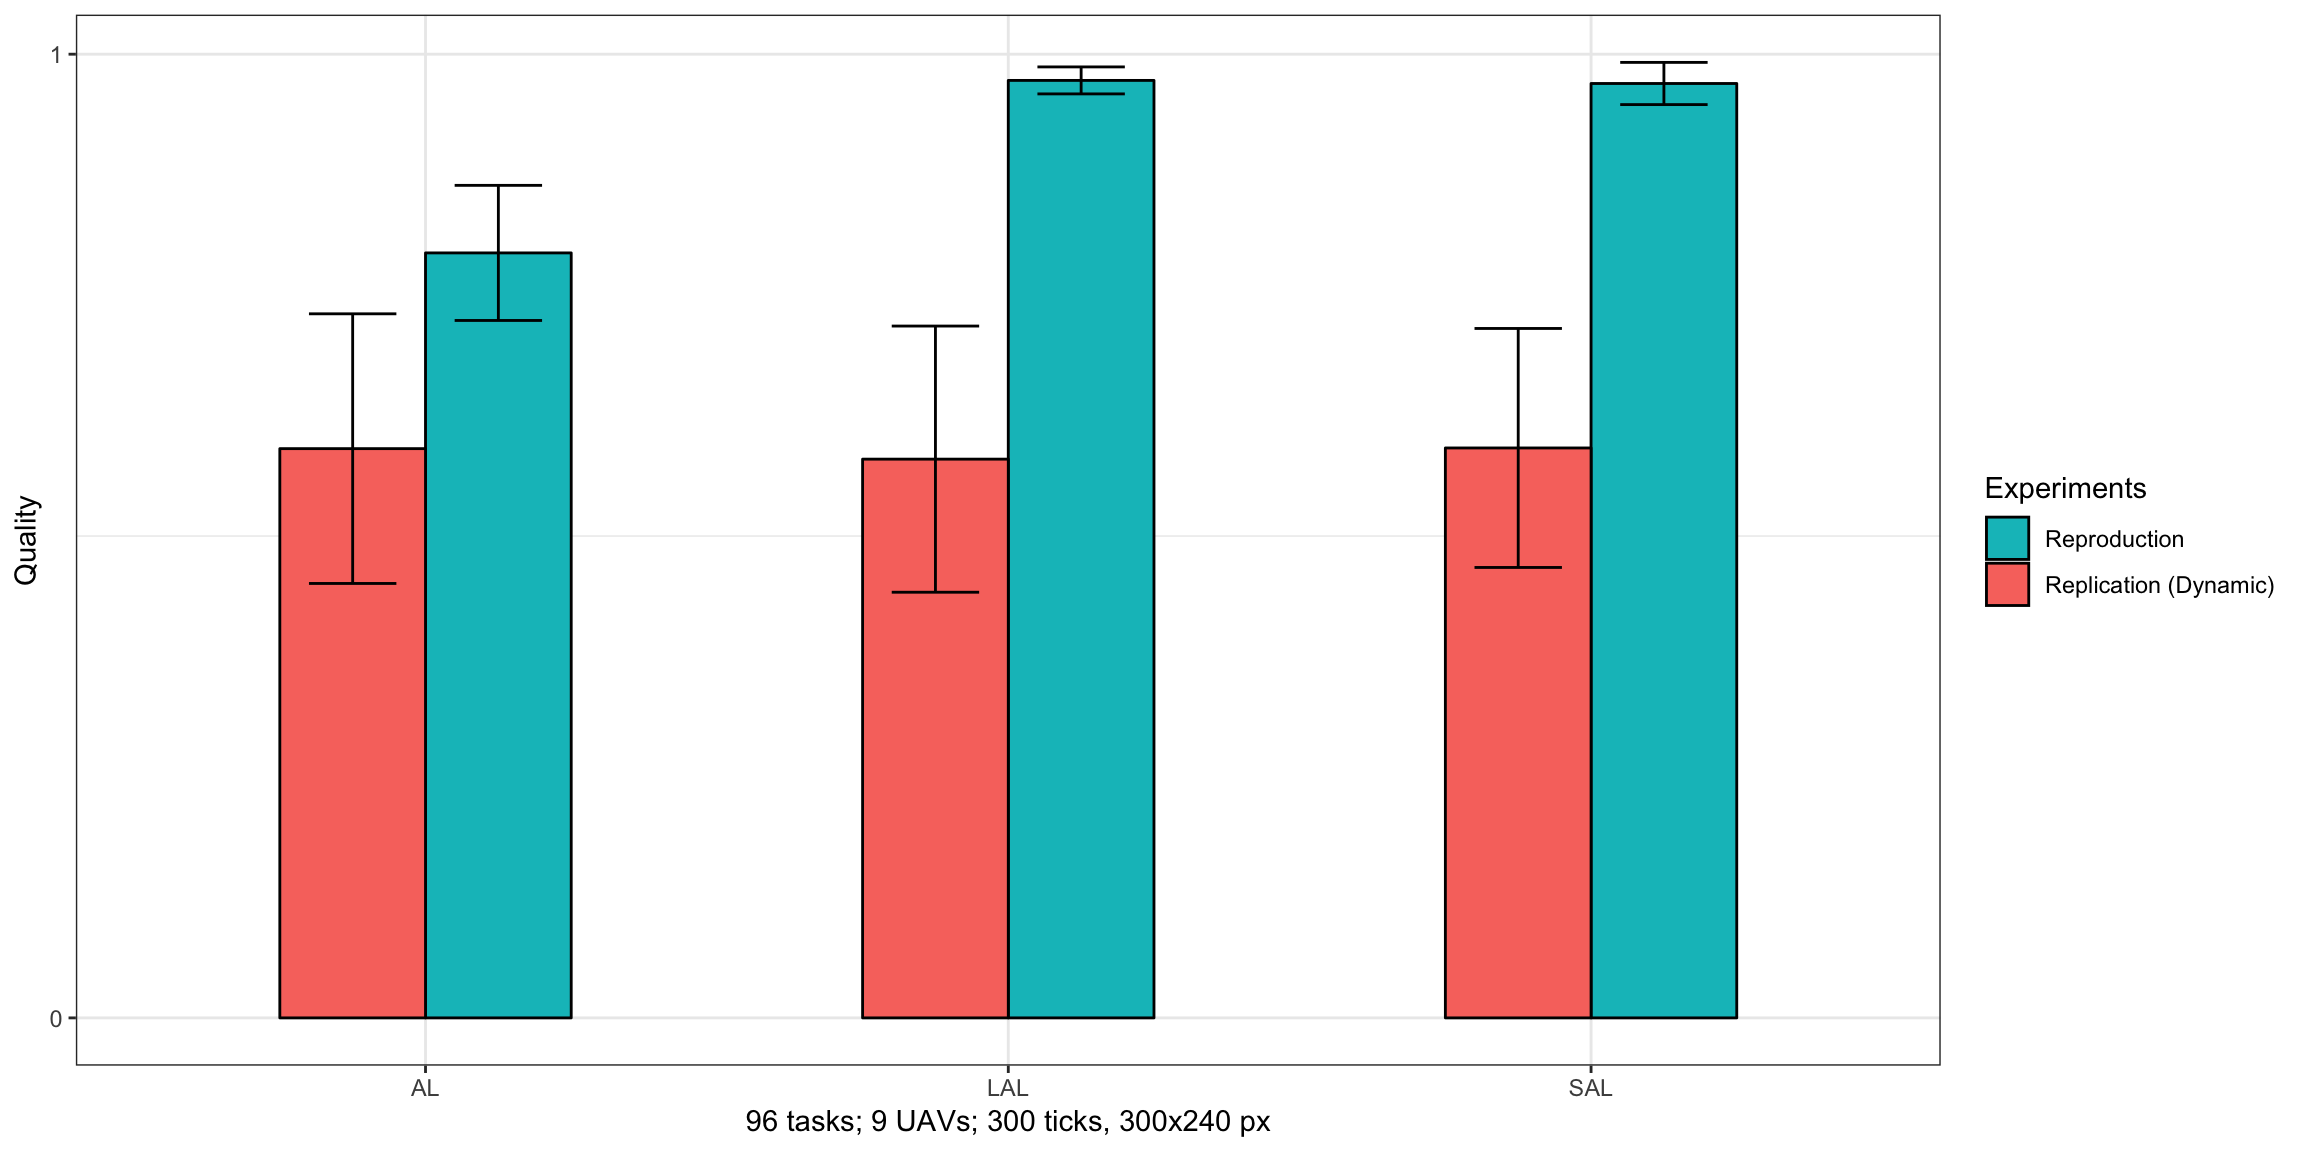
\includegraphics[scale=0.15]{fig/quality_orig.png}
		\caption{Quality (96 tasks; 9 UAVs; 300 x 240; 300 ticks)}
		\label{fig:fig03}
	\end{center}
\end{figure}

On another hand, other attributes presented very similar results to the original experiment as the number of messages exchanged, and total reward and time.

The ring network relies on passing a token to each element. Even reducing the number of elements, the number of messages did not reduce because the token runs while it has task available or there is an UAV not visited by the token.

As the total reward is the sum of the UAV capability $k_{ij}$ related to the task finished, and the capability, defined in \cite{MAS07}, is a correlation among distance to the task and the sensor quality, the reduction of one is offset by the other, as confirmed by Figure \ref{fig:fig02}.

\begin{figure}[h!]
	\begin{center}
		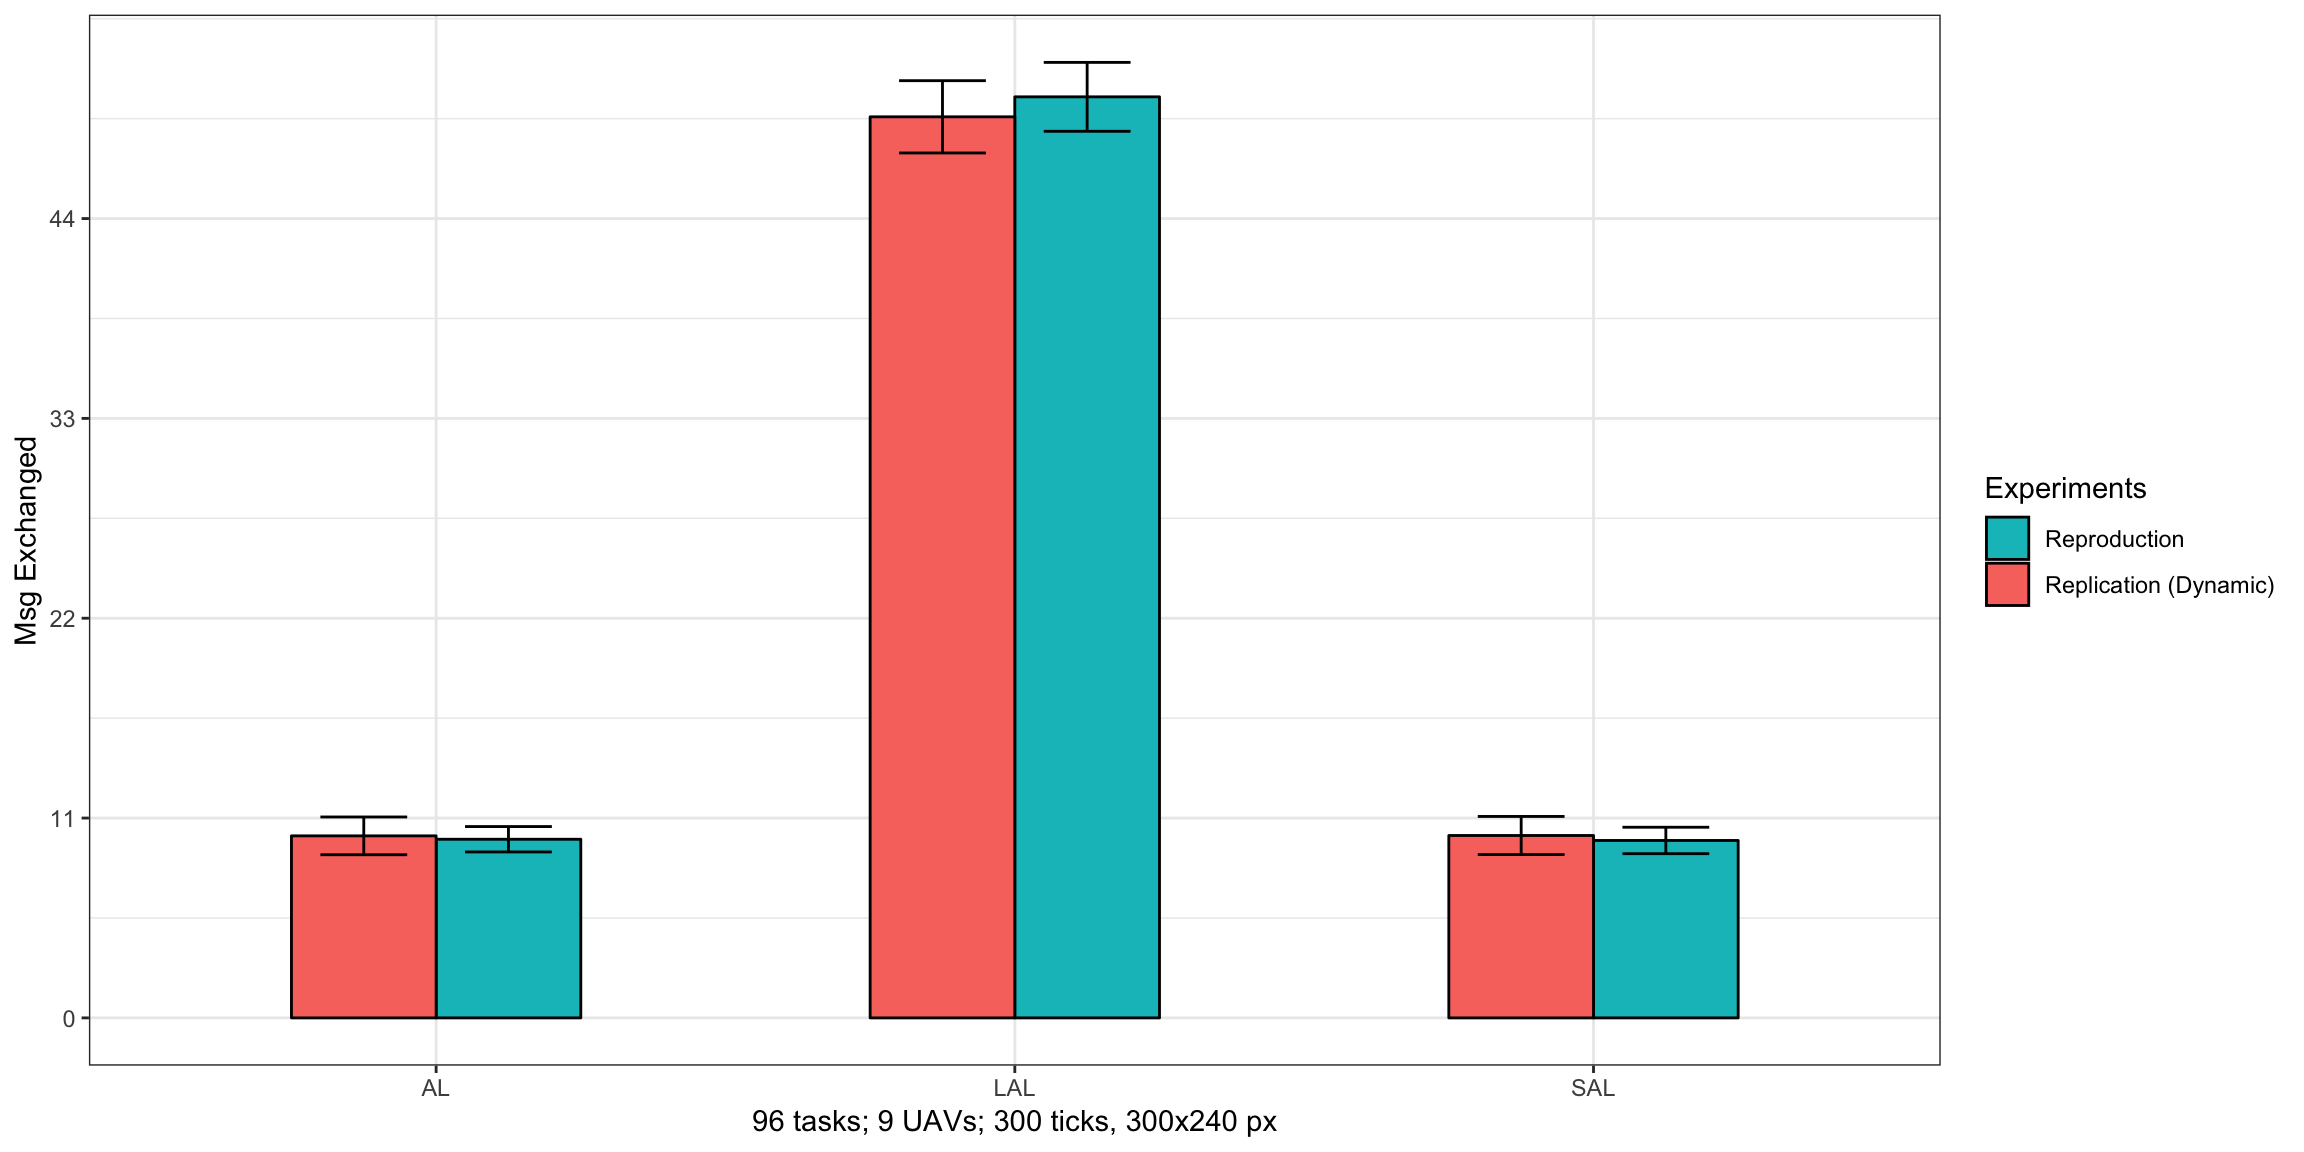
\includegraphics[scale=0.15]{fig/msg_orig.png}
		\caption{Messages exchanged (96 tasks; 9 UAVs; 300 x 240; 300 ticks)}
		\label{fig:fig01}
	\end{center}
\end{figure}

\begin{figure}[h!]
	\begin{center}
		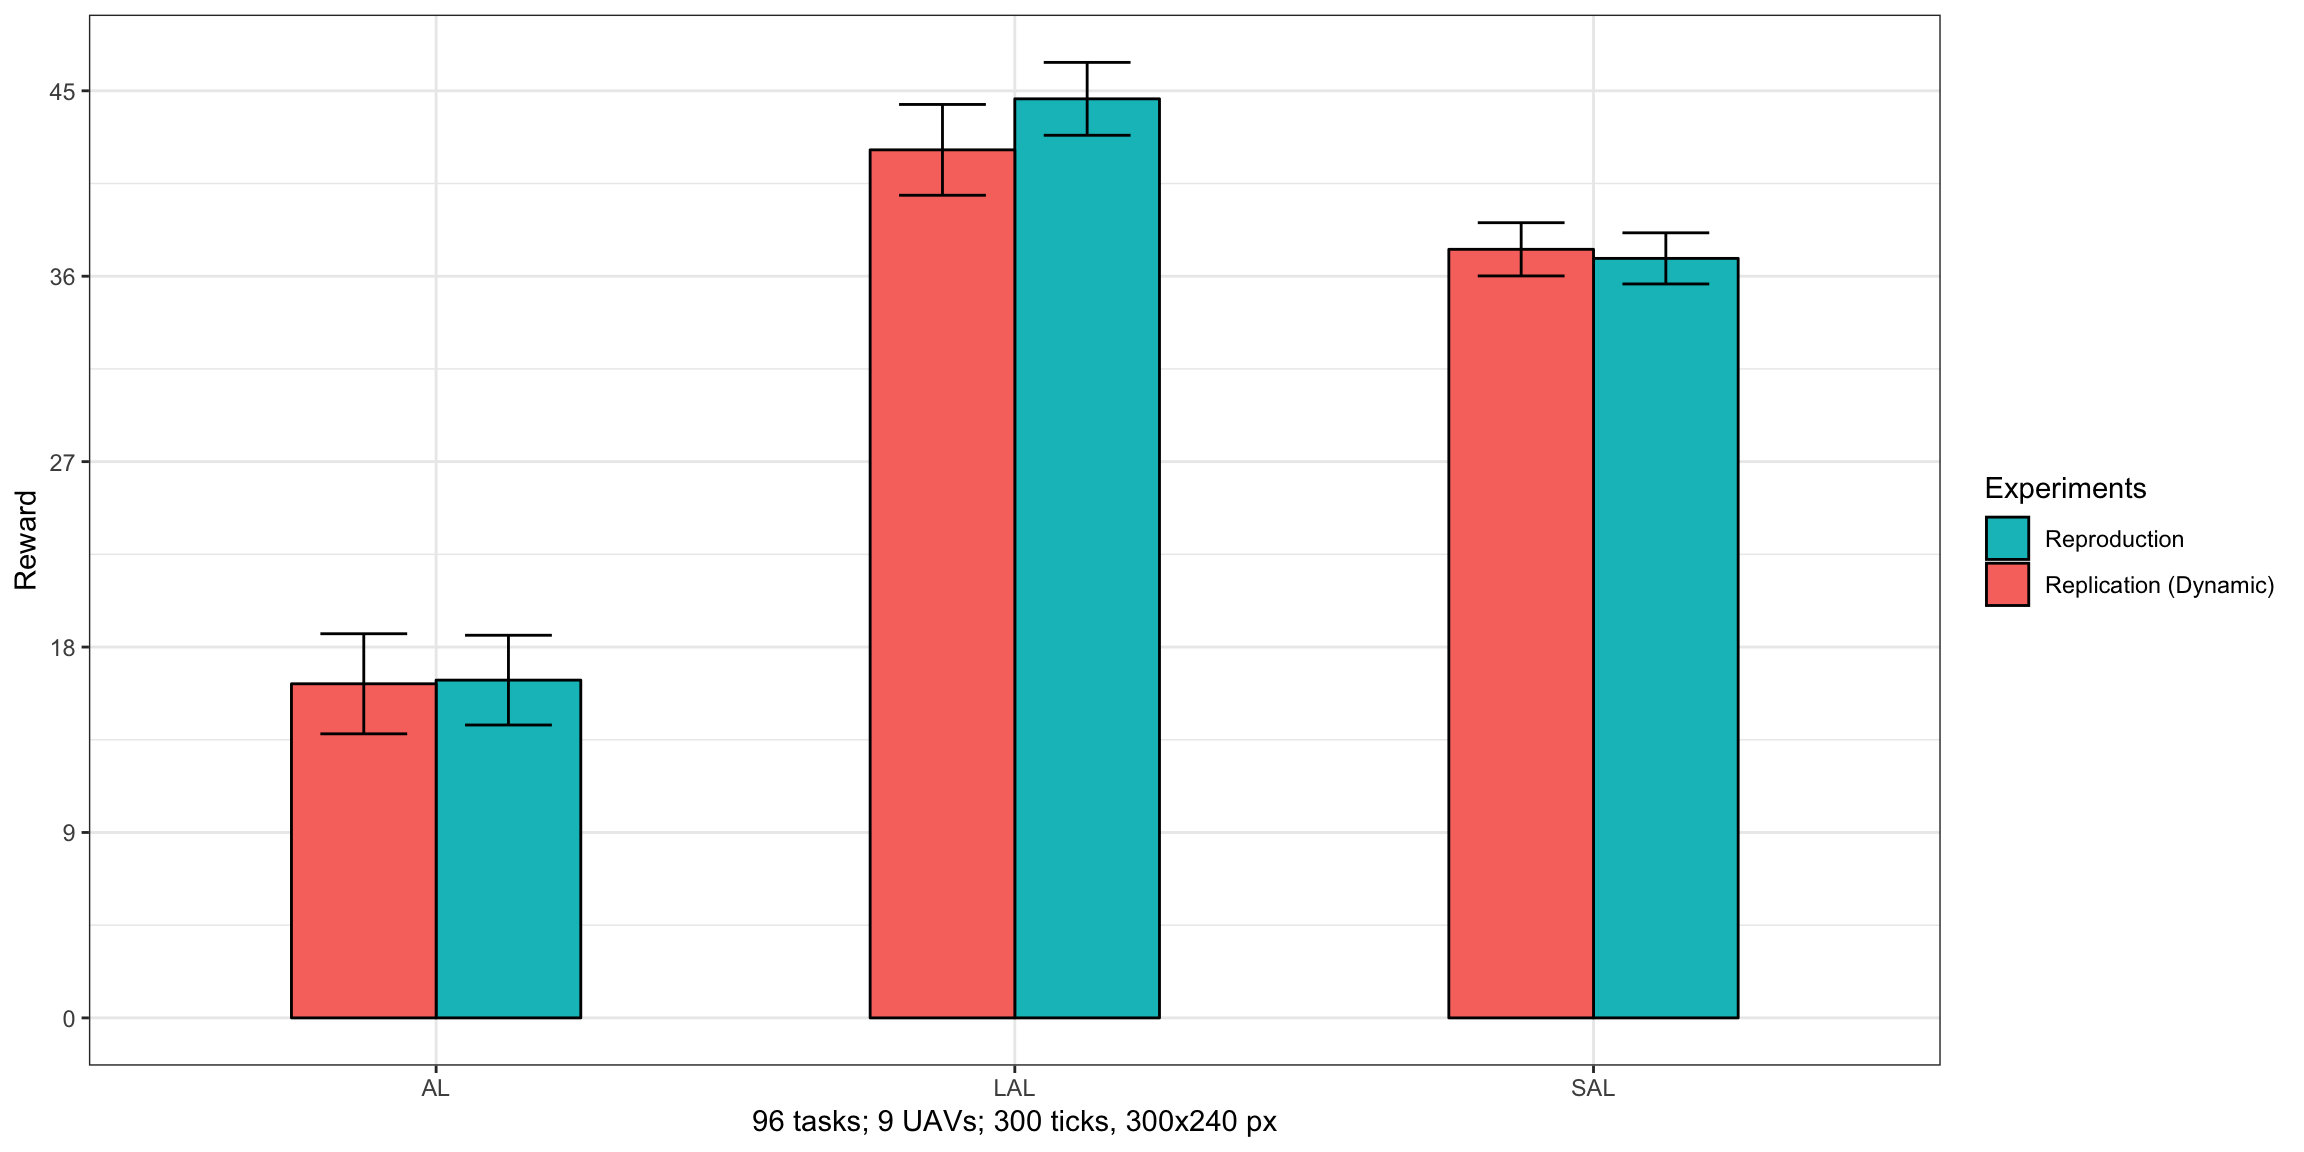
\includegraphics[scale=0.15]{fig/reward_orig.png}
		\caption{Total Reward (96 tasks; 9 UAVs; 300 x 240; 300 ticks)}
		\label{fig:fig02}
	\end{center}
\end{figure}

\begin{figure}[h!]
	\begin{center}
		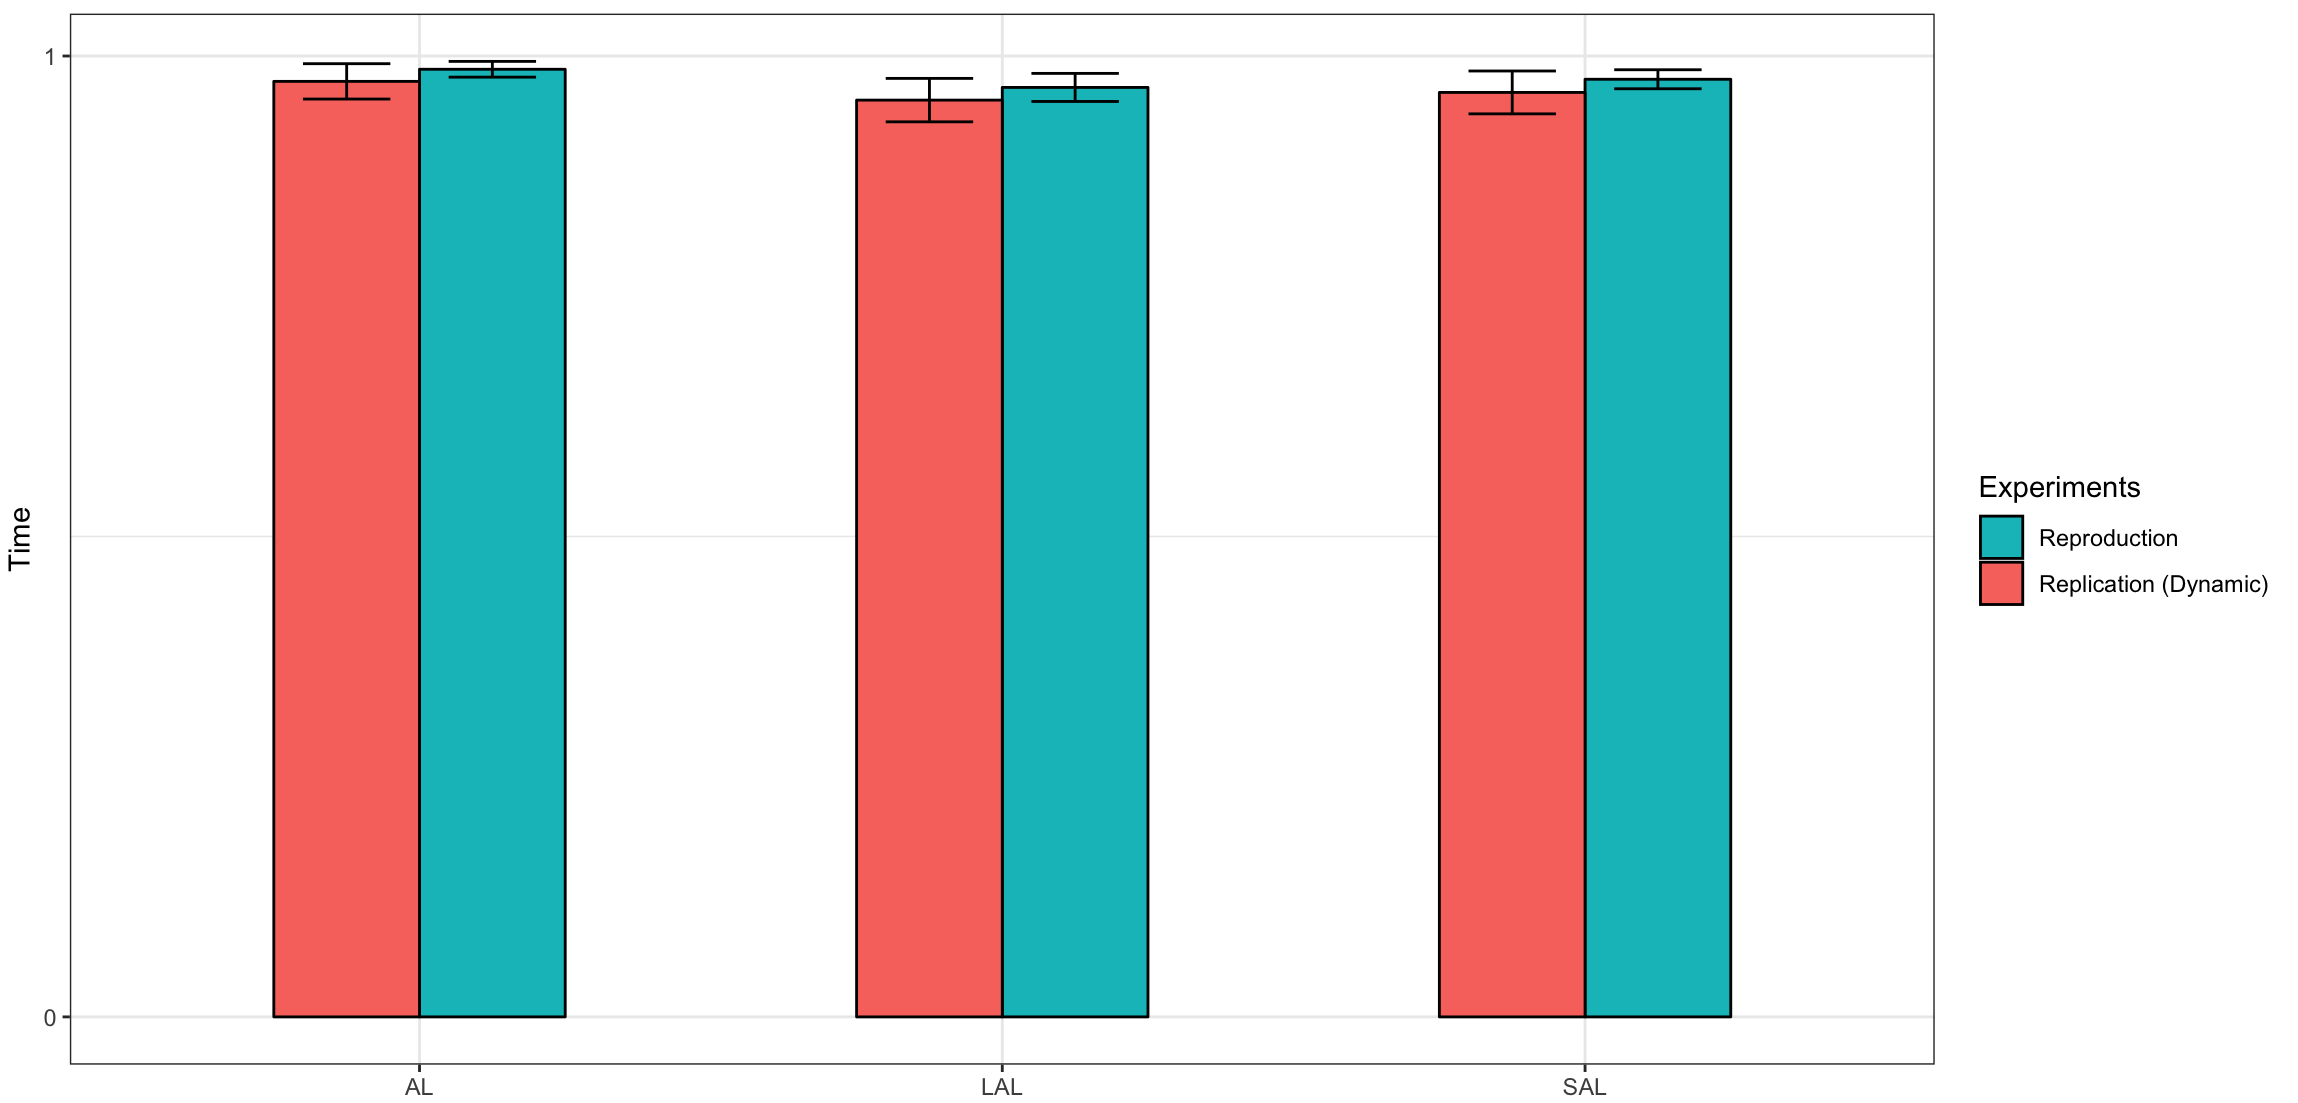
\includegraphics[scale=0.15]{fig/time_orig.png}
		\caption{Time Elapsed (96 tasks; 9 UAVs; 300 x 240; 300 ticks)}
		\label{fig:time}
	\end{center}
\end{figure}

The time measurement was done in percentage of total mission time (in ticks) utilization. This total time was kept the same compared of original experiment and equals to 300 ticks. The result obtained was equivalent, considering the standard deviation (see Figure \ref{fig:time}). It is explained because the dynamic scenario ensures at least one UAV and this agent spends the most of time (in ticks) available to execute the tasks allocated to it.

According to what was presented in \cite{MAS07} and \cite{ferreira2007swarm}, the more suitable value for $stimulus$ attribute is $0.6$. However, during the replications, we investigated different values. The resulting differences were not significant compared to those using the original $stimulus$ value in a static context reproduction. Therefore, all final results obtained in this section were based on the $stimulus = 0.6$